\documentclass{ximera}

%\usepackage{todonotes}

\newcommand{\todo}{}

\usepackage{esint} % for \oiint
\ifxake%%https://math.meta.stackexchange.com/questions/9973/how-do-you-render-a-closed-surface-double-integral
\renewcommand{\oiint}{{\large\bigcirc}\kern-1.56em\iint}
\fi


\graphicspath{
  {./}
  {ximeraTutorial/}
  {basicPhilosophy/}
  {functionsOfSeveralVariables/}
  {normalVectors/}
  {lagrangeMultipliers/}
  {vectorFields/}
  {greensTheorem/}
  {shapeOfThingsToCome/}
  {dotProducts/}
  {partialDerivativesAndTheGradientVector/}
  {../productAndQuotientRules/exercises/}
  {../normalVectors/exercisesParametricPlots/}
  {../continuityOfFunctionsOfSeveralVariables/exercises/}
  {../partialDerivativesAndTheGradientVector/exercises/}
  {../directionalDerivativeAndChainRule/exercises/}
  {../commonCoordinates/exercisesCylindricalCoordinates/}
  {../commonCoordinates/exercisesSphericalCoordinates/}
  {../greensTheorem/exercisesCurlAndLineIntegrals/}
  {../greensTheorem/exercisesDivergenceAndLineIntegrals/}
  {../shapeOfThingsToCome/exercisesDivergenceTheorem/}
  {../greensTheorem/}
  {../shapeOfThingsToCome/}
  {../separableDifferentialEquations/exercises/}
  {vectorFields/}
}

\newcommand{\mooculus}{\textsf{\textbf{MOOC}\textnormal{\textsf{ULUS}}}}

\usepackage{tkz-euclide}
\usepackage{tikz}
\usepackage{tikz-cd}
\usetikzlibrary{arrows}
\tikzset{>=stealth,commutative diagrams/.cd,
  arrow style=tikz,diagrams={>=stealth}} %% cool arrow head
\tikzset{shorten <>/.style={ shorten >=#1, shorten <=#1 } } %% allows shorter vectors

\usetikzlibrary{backgrounds} %% for boxes around graphs
\usetikzlibrary{shapes,positioning}  %% Clouds and stars
\usetikzlibrary{matrix} %% for matrix
\usepgfplotslibrary{polar} %% for polar plots
\usepgfplotslibrary{fillbetween} %% to shade area between curves in TikZ
%\usetkzobj{all}
\usepackage[makeroom]{cancel} %% for strike outs
%\usepackage{mathtools} %% for pretty underbrace % Breaks Ximera
%\usepackage{multicol}
\usepackage{pgffor} %% required for integral for loops



%% http://tex.stackexchange.com/questions/66490/drawing-a-tikz-arc-specifying-the-center
%% Draws beach ball
\tikzset{pics/carc/.style args={#1:#2:#3}{code={\draw[pic actions] (#1:#3) arc(#1:#2:#3);}}}



\usepackage{array}
\setlength{\extrarowheight}{+.1cm}
\newdimen\digitwidth
\settowidth\digitwidth{9}
\def\divrule#1#2{
\noalign{\moveright#1\digitwidth
\vbox{\hrule width#2\digitwidth}}}




% \newcommand{\RR}{\mathbb R}
% \newcommand{\R}{\mathbb R}
% \newcommand{\N}{\mathbb N}
% \newcommand{\Z}{\mathbb Z}

\newcommand{\sagemath}{\textsf{SageMath}}


%\renewcommand{\d}{\,d\!}
%\renewcommand{\d}{\mathop{}\!d}
%\newcommand{\dd}[2][]{\frac{\d #1}{\d #2}}
%\newcommand{\pp}[2][]{\frac{\partial #1}{\partial #2}}
% \renewcommand{\l}{\ell}
%\newcommand{\ddx}{\frac{d}{\d x}}

% \newcommand{\zeroOverZero}{\ensuremath{\boldsymbol{\tfrac{0}{0}}}}
%\newcommand{\inftyOverInfty}{\ensuremath{\boldsymbol{\tfrac{\infty}{\infty}}}}
%\newcommand{\zeroOverInfty}{\ensuremath{\boldsymbol{\tfrac{0}{\infty}}}}
%\newcommand{\zeroTimesInfty}{\ensuremath{\small\boldsymbol{0\cdot \infty}}}
%\newcommand{\inftyMinusInfty}{\ensuremath{\small\boldsymbol{\infty - \infty}}}
%\newcommand{\oneToInfty}{\ensuremath{\boldsymbol{1^\infty}}}
%\newcommand{\zeroToZero}{\ensuremath{\boldsymbol{0^0}}}
%\newcommand{\inftyToZero}{\ensuremath{\boldsymbol{\infty^0}}}



% \newcommand{\numOverZero}{\ensuremath{\boldsymbol{\tfrac{\#}{0}}}}
% \newcommand{\dfn}{\textbf}
% \newcommand{\unit}{\,\mathrm}
% \newcommand{\unit}{\mathop{}\!\mathrm}
% \newcommand{\eval}[1]{\bigg[ #1 \bigg]}
% \newcommand{\seq}[1]{\left( #1 \right)}
% \renewcommand{\epsilon}{\varepsilon}
% \renewcommand{\phi}{\varphi}


% \renewcommand{\iff}{\Leftrightarrow}

% \DeclareMathOperator{\arccot}{arccot}
% \DeclareMathOperator{\arcsec}{arcsec}
% \DeclareMathOperator{\arccsc}{arccsc}
% \DeclareMathOperator{\si}{Si}
% \DeclareMathOperator{\scal}{scal}
% \DeclareMathOperator{\sign}{sign}


%% \newcommand{\tightoverset}[2]{% for arrow vec
%%   \mathop{#2}\limits^{\vbox to -.5ex{\kern-0.75ex\hbox{$#1$}\vss}}}
% \newcommand{\arrowvec}[1]{{\overset{\rightharpoonup}{#1}}}
% \renewcommand{\vec}[1]{\arrowvec{\mathbf{#1}}}
% \renewcommand{\vec}[1]{{\overset{\boldsymbol{\rightharpoonup}}{\mathbf{#1}}}}

% \newcommand{\point}[1]{\left(#1\right)} %this allows \vector{ to be changed to \vector{ with a quick find and replace
% \newcommand{\pt}[1]{\mathbf{#1}} %this allows \vec{ to be changed to \vec{ with a quick find and replace
% \newcommand{\Lim}[2]{\lim_{\point{#1} \to \point{#2}}} %Bart, I changed this to point since I want to use it.  It runs through both of the exercise and exerciseE files in limits section, which is why it was in each document to start with.

% \DeclareMathOperator{\proj}{\mathbf{proj}}
% \newcommand{\veci}{{\boldsymbol{\hat{\imath}}}}
% \newcommand{\vecj}{{\boldsymbol{\hat{\jmath}}}}
% \newcommand{\veck}{{\boldsymbol{\hat{k}}}}
% \newcommand{\vecl}{\vec{\boldsymbol{\l}}}
% \newcommand{\uvec}[1]{\mathbf{\hat{#1}}}
% \newcommand{\utan}{\mathbf{\hat{t}}}
% \newcommand{\unormal}{\mathbf{\hat{n}}}
% \newcommand{\ubinormal}{\mathbf{\hat{b}}}

% \newcommand{\dotp}{\bullet}
% \newcommand{\cross}{\boldsymbol\times}
% \newcommand{\grad}{\boldsymbol\nabla}
% \newcommand{\divergence}{\grad\dotp}
% \newcommand{\curl}{\grad\cross}
%\DeclareMathOperator{\divergence}{divergence}
%\DeclareMathOperator{\curl}[1]{\grad\cross #1}
% \newcommand{\lto}{\mathop{\longrightarrow\,}\limits}

% \renewcommand{\bar}{\overline}

\colorlet{textColor}{black}
\colorlet{background}{white}
\colorlet{penColor}{blue!50!black} % Color of a curve in a plot
\colorlet{penColor2}{red!50!black}% Color of a curve in a plot
\colorlet{penColor3}{red!50!blue} % Color of a curve in a plot
\colorlet{penColor4}{green!50!black} % Color of a curve in a plot
\colorlet{penColor5}{orange!80!black} % Color of a curve in a plot
\colorlet{penColor6}{yellow!70!black} % Color of a curve in a plot
\colorlet{fill1}{penColor!20} % Color of fill in a plot
\colorlet{fill2}{penColor2!20} % Color of fill in a plot
\colorlet{fillp}{fill1} % Color of positive area
\colorlet{filln}{penColor2!20} % Color of negative area
\colorlet{fill3}{penColor3!20} % Fill
\colorlet{fill4}{penColor4!20} % Fill
\colorlet{fill5}{penColor5!20} % Fill
\colorlet{gridColor}{gray!50} % Color of grid in a plot

\newcommand{\surfaceColor}{violet}
\newcommand{\surfaceColorTwo}{redyellow}
\newcommand{\sliceColor}{greenyellow}




\pgfmathdeclarefunction{gauss}{2}{% gives gaussian
  \pgfmathparse{1/(#2*sqrt(2*pi))*exp(-((x-#1)^2)/(2*#2^2))}%
}


%%%%%%%%%%%%%
%% Vectors
%%%%%%%%%%%%%

%% Simple horiz vectors
\renewcommand{\vector}[1]{\left\langle #1\right\rangle}


%% %% Complex Horiz Vectors with angle brackets
%% \makeatletter
%% \renewcommand{\vector}[2][ , ]{\left\langle%
%%   \def\nextitem{\def\nextitem{#1}}%
%%   \@for \el:=#2\do{\nextitem\el}\right\rangle%
%% }
%% \makeatother

%% %% Vertical Vectors
%% \def\vector#1{\begin{bmatrix}\vecListA#1,,\end{bmatrix}}
%% \def\vecListA#1,{\if,#1,\else #1\cr \expandafter \vecListA \fi}

%%%%%%%%%%%%%
%% End of vectors
%%%%%%%%%%%%%

%\newcommand{\fullwidth}{}
%\newcommand{\normalwidth}{}



%% makes a snazzy t-chart for evaluating functions
%\newenvironment{tchart}{\rowcolors{2}{}{background!90!textColor}\array}{\endarray}

%%This is to help with formatting on future title pages.
\newenvironment{sectionOutcomes}{}{}



%% Flowchart stuff
%\tikzstyle{startstop} = [rectangle, rounded corners, minimum width=3cm, minimum height=1cm,text centered, draw=black]
%\tikzstyle{question} = [rectangle, minimum width=3cm, minimum height=1cm, text centered, draw=black]
%\tikzstyle{decision} = [trapezium, trapezium left angle=70, trapezium right angle=110, minimum width=3cm, minimum height=1cm, text centered, draw=black]
%\tikzstyle{question} = [rectangle, rounded corners, minimum width=3cm, minimum height=1cm,text centered, draw=black]
%\tikzstyle{process} = [rectangle, minimum width=3cm, minimum height=1cm, text centered, draw=black]
%\tikzstyle{decision} = [trapezium, trapezium left angle=70, trapezium right angle=110, minimum width=3cm, minimum height=1cm, text centered, draw=black]


\title{Theory}

\begin{document}

\begin{abstract}
the rational story
\end{abstract}
\maketitle









Rational functions are quotients or fractions of polynomials.  (Polynomials are rational functions, since they can be written in a fraction form with $1$ as the denominator.)  So, it is not surprising that analyzing rational function follows the same plan as for polynomials.



















\begin{definition} \item \textbf{\textcolor{green!50!black}{Rational Function}}  


A \textbf{rational function} is a function that can be represented by a formula of the form


\[   R(x) = \frac{a_n x^n + a_{n-1} x^{n-1} + \cdots + a_2 x^2 + a_1 x + a_0}{b_m x^m + b_{m-1} x^{m-1} + \cdots + b_2 x^2 + b_1 x + b_0}        \]

where the $a_i$ and $b_i$ are real numbers with $a_n \ne 0$ and $b_m \ne 0$.


\end{definition}



$\blacktriangleright$ \textbf{\textcolor{red!10!blue!90!}{Domain:}}  The natural or implied domain of a rational function is all real numbers, except those that make the denominator equal to $0$.  



Of course, any particular rational function may be defined with a stated subset of the real numbers as the domain, in which case we  say that it is a \textbf{restricted} rational function.








Following our analysis of polynomials, we would like to factor, collect common factors, and reduce or simplify.


\[  R(x)  = \frac{a (x - r_k)^{e_k} (x - r_{k-1})^{e_{k-1}} \cdots (x - r_1)^{e_1} }{b (x - s_h)^{f_h} (x - s_{h-1})^{f_{h-1}} \cdots (x - s_1)^{f_1}}            \]


Here, the roots are distinct, which means that  $r_i \ne r_j$ when $i \ne j$, and $s_i \ne s_j$ when $i \ne j$, and $r_i \ne s_j$ for all $i$ and $j$.



\begin{warning}   \textbf{\textcolor{red!80!black}{Common Roots}} \\

The formula for a rational function could have a root in common between the polynomials in the numerator and denominator.

In this case, we would like to factor out the common factors and simplify the formula.

If this simplification results in the removal of a factor from the denominator, we must remember that the corresponding root is still excluded from the domain as the original formula excluded it.

The domain is determined by the original definition of the function, not by any simplification.

\end{warning}





\begin{example}

Let $R$ be defined as follows.


\[   R(x) = \frac{(x-3)(x-1)}{x-1}            \]


Just thinking algebraically, we might simplify this to $R(x) = x-3$. However, thinking functionally, these two formulas have different natural or implied domains.


We have to remember that that the domain of $R$ is still $\left( -\infty, \answer{1} \right) \cup \left( \answer{1},\infty \right)$ no mater what algebraic modifications have been made.

$R(x)$ and $p(x) = x-3$ are different functions, since they have different natural domains. $R(x) = x - 3$, provided we note that $x \ne 1$.


The graphs of $R(x)$ and $p(x) = x-3$ are the same, except at $x=1$.  The graph of $p(x) = x-3$ includes the point $(1, -2)$, while the graph of $R(x)$ omits this point.



The graph of $p(x) = x-3$ is a line, while the graph is the same line with a hole in it at $\left( 1, \answer{-2} \right)$.












Graph of $y = R(x)$.


\begin{image}
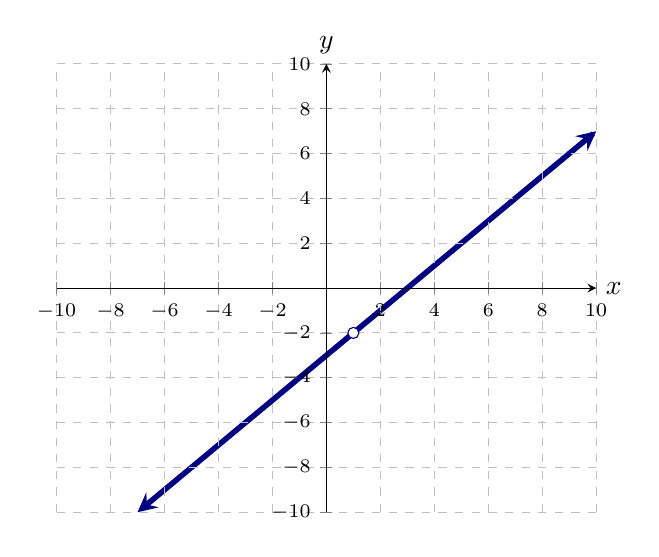
\begin{tikzpicture}
  \begin{axis}[
            domain=-10:10, ymax=10, xmax=10, ymin=-10, xmin=-10,
            axis lines =center, xlabel=$x$, ylabel=$y$, grid = major, grid style={dashed},
            ytick={-10,-8,-6,-4,-2,2,4,6,8,10},
            xtick={-10,-8,-6,-4,-2,2,4,6,8,10},
            yticklabels={$-10$,$-8$,$-6$,$-4$,$-2$,$2$,$4$,$6$,$8$,$10$}, 
            xticklabels={$-10$,$-8$,$-6$,$-4$,$-2$,$2$,$4$,$6$,$8$,$10$},
            ticklabel style={font=\scriptsize},
            every axis y label/.style={at=(current axis.above origin),anchor=south},
            every axis x label/.style={at=(current axis.right of origin),anchor=west},
            axis on top
          ]
          

            \addplot [line width=2, penColor, smooth,samples=100,domain=(-7:10),<->] {x-3};

          	\addplot[color=penColor,fill=white,only marks,mark=*] coordinates{(1,-2)};


           

  \end{axis}
\end{tikzpicture}
\end{image}



$1$ does not cause a problem for $x-3$, but that isn't the formula for $R$. \\

$R(x) = \frac{(x-3)(x-1)}{(x-1)}$ is equal to $x-3$, provided $x \ne 1$.  We cannot reinsert $1$ after simplifying.




\end{example}

We prefer working with a simplified formula.  We just need to keep track of how simplifying affects factors.






\textbf{\textcolor{red!80!black}{Assuming a simplified formula...}} \\


\textbf{\textcolor{red!80!black}{Note:}} A simplified formula assures us that the zeros of the numerator polynomial are all different from the zeros of the denominator polynomial. (Otherwise, we would have removed the common factors.) \\





$\blacktriangleright$ \textbf{\textcolor{red!10!blue!90!}{Roots and Zeros:}} \\
   Zeros or Roots of a rational function are the zeros or roots of the numerator polynomial.  A polynomial function behaves in one of two ways around a root.

\begin{itemize}
\item If the multiplicity is odd then the function changes sign over the root.  The graph crosses over the horizontal axis at the corresponding intercept.
\item If the multiplicity is even then the function does not change sign over the root.  The graph does not cross over the horizontal axis at the corresponding intercept. Instead, it bounces back in the direction from which it came.
\end{itemize}






$\blacktriangleright$ \textbf{\textcolor{red!10!blue!90!}{Singularities:}} \\
Singularities of a rational function are the zeros of the denominator polynomial.  Vertical asymptotes usually represent these types of singularities graphically.

\begin{itemize}
\item If the multiplicity is odd then the function changes sign over the singularity.  The graph moves to the other end of the corresponding vertical asymptote.
\item If the multiplicity is even then the function does not change sign over the singularity.  The graph does not move to the other end of the corresponding vertical asymptote. 
\end{itemize}




$\blacktriangleright$ \textbf{\textcolor{red!10!blue!90!}{Hole:}} \\
Another type of singularity for rational functions is a hole. If a common factor between the numerator and denominator have the same multiplicity, then they will be completely removed from the formula upon simplification.  In this case, the rational function behaves nicely, except that particular number is removed from the domain.  We have a hole in the graph.  The new, simplified formula has a value for the missing factors.  However, we cannot use it, because the factors were initially there, thus removing the zero from the domain.  Therefore, we end up with a hole in the graph. \\



\textbf{Note:} Remember, the original formula dictates the domain. The simplified form might have a factor in the numerator, indicating a zero. However, if the original formula also had a matching denominator factor, then there will be a hole in the graph rather than an intercept. 






\begin{definition} \textbf{\textcolor{green!50!black}{Removeable Singularity}}

If a function can be defined at a single nondomain number to remove a singularity, then that singularity is said to be \textbf{removeable}.

\end{definition}

\textbf{Note:} Removeable singularities show up as holes in the graph.  There is no domain number corresponding to the point that has been removed. The hole can be filled by inserting a single point.  The singularity can be removed by defining the function at a single number.  This would ``remove'' the singularity. \\

Of course ``fixing'' the hole of singularity creates a new and different function.  This new and different function is exactly the same as the original function, except for one single ordered pair.







\begin{definition} \textbf{\textcolor{green!50!black}{Removeable Discontinuity}}

If a function can be redefined at a single domain number to remove a discontinuity, then that discontiuity is said to be \textbf{removeable}.

\end{definition}

\textbf{Note:} Removeable discontintinuities are just like removeable singlularities, except there is a point on the graph.  It is just somewhere else besides filling in the hole.  The hole or discontinuity can be ``removed'' by re-defining the function at that one domain number to fill in the hole.\\

Of course moving the dot and ``filling in'' the hole of discontinuity creates a new and different function.  This new and different function is exactly the same as the original function, except for one single pair.






\begin{example}  Missing Intercept

\[     R(x) = \frac{(x+4)(x-5)^2}{(x-5)(x-7)}     \]

reduces to 

\[     R(x) = \frac{(x+4)(x-5)}{(x-7)}     \]


It appears that $R(x)$ has $5$ as a root and $(5,0)$ as an intercept for the graph.  However, the original formula for $R$ removed $5$ from the domain.  Therefore, the graph has a missing intercept. $(5,0)$ is plotted as a hollow dot.



We could define $R(5)=0$ and then the hole would disappear from the graph.  The singularity would disappear from the function. Therefore, $5$ is a removeable singularity of $R$.


\end{example}

We must always remember the original formula when it comes to the domain.  Simplification cannot change the domain. \\





$\blacktriangleright$ \textbf{\textcolor{red!10!blue!90!}{Continuity:}} \\
For the most part, rational functions are relatively nice functions.  They are continuous everywhere in their domain.  They have no discontinuities.  The singularities correspond to vertical asymptotes or removeable singularities, both of which we understand.  \\

Of course, we are always on the lookout for common factors, which are represented with holes in the graph.








$\blacktriangleright$ \textbf{\textcolor{red!10!blue!90!}{End-Behavior:}} \\
In addition to identifying zeros, roots, dicontinuities, singularities, maximums, and minimums, we would also like to describe any pattern the function takes on as the domain heads to infinity or negative infinity.  These patterns we call the ``end-behavior'' of the function.  \\

In the case of a rational function there are three types of end-behavior, which can be ascertained by comparing the leading terms of the polynomials in the numerator and denominator.


\begin{itemize}
\item If the degrees of the leading terms are equal then the end-behavior is the quotient of the leading coefficients.


\[   \lim\limits_{x \to \infty} R(x) = \frac{a_n x^n + a_{n-1} x^{n-1} + \cdots + a_2 x^2 + a_1 x + a_0}{b_n x^n + b_{n-1} x^{n-1} + \cdots + b_2 x^2 + b_1 x + b_0}  = \frac{a_n}{b_n}      \]


\[   \lim\limits_{x \to -\infty} R(x) = \frac{a_n x^n + a_{n-1} x^{n-1} + \cdots + a_2 x^2 + a_1 x + a_0}{b_n x^n + b_{n-1} x^{n-1} + \cdots + b_2 x^2 + b_1 x + b_0}  = \frac{a_n}{b_n}      \]



\item If the degree of numerator polynomial is greater than the degree of the denominator polynomial, then the rational function becomes unbounded.

If $n > m$, then 

\[   \lim\limits_{x \to \infty} R(x) = \frac{a_n x^n + a_{n-1} x^{n-1} + \cdots + a_2 x^2 + a_1 x + a_0}{b_m x^m + b_{m-1} x^{m-1} + \cdots + b_2 x^2 + b_1 x + b_0} = \pm\infty       \]


\[   \lim\limits_{x \to -\infty} R(x) = \frac{a_n x^n + a_{n-1} x^{n-1} + \cdots + a_2 x^2 + a_1 x + a_0}{b_m x^m + b_{m-1} x^{m-1} + \cdots + b_2 x^2 + b_1 x + b_0} = \pm\infty       \]

The sign depends on the signs of the leading coefficients and the degrees of the polynomials.


\item If the degree of denominator polynomial is greater than the degree of the numerator polynomial, then the rational function tends to $0$.

If $n < m$, then 

\[   \lim\limits_{x \to \infty} R(x) = \frac{a_n x^n + a_{n-1} x^{n-1} + \cdots + a_2 x^2 + a_1 x + a_0}{b_m x^m + b_{m-1} x^{m-1} + \cdots + b_2 x^2 + b_1 x + b_0} = 0      \]


\[   \lim\limits_{x \to -\infty} R(x) = \frac{a_n x^n + a_{n-1} x^{n-1} + \cdots + a_2 x^2 + a_1 x + a_0}{b_m x^m + b_{m-1} x^{m-1} + \cdots + b_2 x^2 + b_1 x + b_0} = 0      \]

\end{itemize}
















$\blacktriangleright$ \textbf{\textcolor{red!10!blue!90!}{Graph:}} \\
Graphs of rational functions are nice.  They are smooth.  They do not have corners or spikes or jump breaks. They do have vertical asymptotes, which we understand.


Once we have the roots of the numerator and denominator polynomials, then we can plot the intercepts and asymptotes.  Then we can smoothly connect everything according to their multiplicities and have a pretty good sketch of the shape of the graph.

With a basic general shape, we can estimate critical numbers and identify the type of extrema values. 

Of course, we are always on the lookout for common factors, which are represented with holes in the graph. \\




$\blacktriangleright$ \textbf{\textcolor{red!10!blue!90!}{Extrema:}} \\
If we have a derivative, then we can attempt to locate exact values of critical numbers.  Without the derivative, we turn to technology for some assistance in approximating critical numbers.




$\blacktriangleright$ \textbf{\textcolor{red!10!blue!90!}{Rate of Change:}} \\
The critical numbers and singularities partition the real line into intervals where the rational function increases or decreases.  We can then list these intervals.















\begin{example} Rational Function


Completely analyze $G(t) = \frac{(t+7)(t+5)(t-2)}{(t+4)^2(t-2)}$




\begin{explanation}



The domain is $\left( -\infty, \answer{-4} \right) \cup \left(\answer{-4}, \answer{2} \right) \cup \left( \answer{2}, \infty \right)$.

Let's simplify: $G(t) = \frac{(t+7)(t+5)}{(t+4)^2}$, since $t-2$ is a common factor, since $-4$ and $2$ make the denominator $0$.



The $t-2$ factor is gone in our simplified formula, but $2$ is still not in the domain.  This will visually show up as a hole in the graph.



\begin{itemize}
\item $-7$ is a root of multiplicity $\answer{1}$.  Since this multiplicity is odd, $G$ will change sign through $\answer{-7}$ and the graph will cross at $(-7,0)$.
\item $-5$ is a root of multiplicity $\answer{1}$.  Since this multiplicity is odd, $G$ will change sign through $-5$ and the graph will cross at $(-5,0)$.
\item $-4$ is a singularity of multiplicity $\answer{2}$.  The function is unbounded near $-4$.  This will show up as a vertical asymptote on the graph. Since this multiplicity is even, $G$ will not change sign across $-4$.  The graph will approach the vertical asymptote similarly on both sides.
\item Our simplified version does not have the $t-2$ factor.  Therefore, the graph will not have an intercept nor a vertical asymptote associated with this factor.  It will have a hole at $\left( 2, \answer{\frac{63}{36}} \right)$.
\end{itemize}


The end-behavior of $G$ is $\frac{t^2}{t^2}$.  Therefore, $\lim\limits_{t \to -\infty}G(t) = 1$ and $\lim\limits_{t \to \infty}G(t) = 1$.  The graph has a horizontal asymptote.




Thinking left to right on the number line, $G$ starts off near $1$, which is positive.  It changes signs across $-7$ and becomes negative. It changes signs across $-5$ and becomes positive.  It cannot change sign until $-4$.  Therefore, $G$ becomes positively unbounded on the left side of $-4$.  Across $-4$, $G$ does not change sign.  Therefore, it is again unbounded and positive on the right side of the vertical asymptote.  There are no more zeros or singularities.  So, $G$ cannot change sign again.  Now, it approaches $1$ from above.




\begin{image}
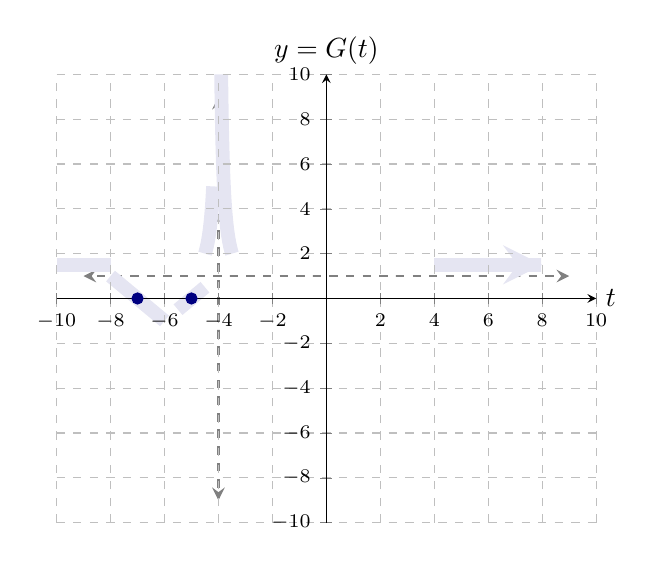
\begin{tikzpicture}
  \begin{axis}[
            domain=-10:10, ymax=10, xmax=10, ymin=-10, xmin=-10,
            axis lines =center, xlabel=$t$, ylabel={$y=G(t)$}, grid = major, grid style={dashed},
            ytick={-10,-8,-6,-4,-2,2,4,6,8,10},
            xtick={-10,-8,-6,-4,-2,2,4,6,8,10},
            yticklabels={$-10$,$-8$,$-6$,$-4$,$-2$,$2$,$4$,$6$,$8$,$10$}, 
            xticklabels={$-10$,$-8$,$-6$,$-4$,$-2$,$2$,$4$,$6$,$8$,$10$},
            ticklabel style={font=\scriptsize},
            every axis y label/.style={at=(current axis.above origin),anchor=south},
            every axis x label/.style={at=(current axis.right of origin),anchor=west},
            axis on top
          ]
          
          	\addplot [line width=1, gray, dashed,samples=200,domain=(-9:9),<->] {1};
          	\addplot [line width=1, gray, dashed,samples=200,domain=(-9:9),<->] ({-4},{x});



            \addplot [line width=5, penColor!10!background, smooth,samples=100,domain=(-8:-6)] {-(x+7)};
            \addplot [line width=5, penColor!10!background, smooth,samples=100,domain=(-5.5:-4.5)] {(x+5)};

            \addplot [line width=5, penColor!10!background, smooth,samples=100,domain=(-4.5:-4.2)] {-1/(x+4)};
            \addplot [line width=5, penColor!10!background, smooth,samples=100,domain=(-3.9:-3.5)] {1/(x+4)};



            \addplot [line width=5, penColor!10!background, smooth,samples=100,domain=(-10:-8)] {1.5)};
            \addplot [line width=5, penColor!10!background, smooth,samples=100,domain=(4:8),->] {1.5)};



          	\addplot[color=penColor,fill=penColor,only marks,mark=*] coordinates{(-7,0)};
          	\addplot[color=penColor,fill=penColor,only marks,mark=*] coordinates{(-5,0)};


           

  \end{axis}
\end{tikzpicture}
\end{image}









The graph is very suggestive that there is a local minimum somewhere around $-5.5$.  






\begin{image}
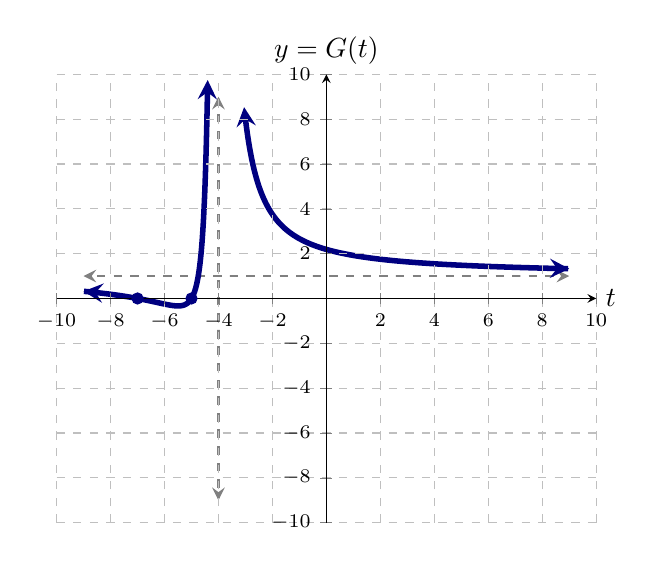
\begin{tikzpicture}
  \begin{axis}[
            domain=-10:10, ymax=10, xmax=10, ymin=-10, xmin=-10,
            axis lines =center, xlabel=$t$, ylabel={$y=G(t)$}, grid = major, grid style={dashed},
            ytick={-10,-8,-6,-4,-2,2,4,6,8,10},
            xtick={-10,-8,-6,-4,-2,2,4,6,8,10},
            yticklabels={$-10$,$-8$,$-6$,$-4$,$-2$,$2$,$4$,$6$,$8$,$10$}, 
            xticklabels={$-10$,$-8$,$-6$,$-4$,$-2$,$2$,$4$,$6$,$8$,$10$},
            ticklabel style={font=\scriptsize},
            every axis y label/.style={at=(current axis.above origin),anchor=south},
            every axis x label/.style={at=(current axis.right of origin),anchor=west},
            axis on top
          ]
          
            \addplot [line width=1, gray, dashed,samples=200,domain=(-9:9),<->] {1};
            \addplot [line width=1, gray, dashed,samples=200,domain=(-9:9),<->] ({-4},{x});


            \addplot [line width=2, penColor, smooth,samples=300,domain=(-9:-4.4),<->] {((x+7)*(x+5))/(x+4)^2};
            \addplot [line width=2, penColor, smooth,samples=300,domain=(-3.05:9),<->] {((x+7)*(x+5))/(x+4)^2};


            \addplot[color=penColor,fill=penColor,only marks,mark=*] coordinates{(-7,0)};
            \addplot[color=penColor,fill=penColor,only marks,mark=*] coordinates{(-5,0)};


           

  \end{axis}
\end{tikzpicture}
\end{image}












With some technology, we can approximate the critical number to be $-5.5$ and the local minimum to be $-0.333$.




\begin{center}
\desmos{st4dfylktg}{400}{300}
\end{center}







\begin{itemize}
\item $G$ decreases on $(-\infty, -5.5]$.
\item $G$ increases on $[-5.5, -4)$.
\item $G$ decreases on $(-4, \infty)$.
\end{itemize}



The local minimum at $-5.5$ is also a global minimum.  There is no global maximum.  There are no local maximums.


\end{explanation}

\end{example}

























\begin{center}
\textbf{\textcolor{green!50!black}{ooooo=-=-=-=-=-=-=-=-=-=-=-=-=ooOoo=-=-=-=-=-=-=-=-=-=-=-=-=ooooo}} \\

more examples can be found by following this link\\ \link[More Examples of Rational Functions]{https://ximera.osu.edu/csccmathematics/precalculus2/precalculus2/rationalFunctions/examples/exampleList}

\end{center}




\end{document}
